
\chapter{Black hole-galaxy co-evolution in the context of quenching}\label{agnfeedback}

The following chapter is split into two parts; in Section \ref{agnfeedback} I investigate the connection between rapid quenching and the presence of an AGN and in Section \ref{intbulgeless} investigate how black holes grow in disk galaxies with merger free evolutionary histories. 

\section{Rapid, recent quenching within a population of Type 2 AGN host galaxies}\label{agnfeedback}

\emph{The work in the following chapter has been published in \citet{smethurst16}.}

With the dominance of rapid, recent quenching for smooth galaxies and the suggested connection between these rates of quenching in mergers with AGN feedback from simulations discussed in Chapter \ref{morph}, I decided to investigate this relation further. By investigating the quenching parameters of a population of AGN host galaxies with \textsc{popstarpy} in comparison to an inactive galaxy control sample I  aim to determine the following: (i) Are galaxies currently hosting an AGN undergoing quenching? (ii) If so, when and at what rate does this quenching occur? (iii) Is this quenching occurring at different times and rates compared to a control sample of inactive galaxies? This builds on the work of \citet{Martin07} but improves significantly on previous techniques.

\subsection{AGN Sample}\label{agnsample}

Type 2 AGN were selected from the \textsc{gz2-galex} sample using a BPT diagram \citep{bpt} using line and continuum strengths for [OIII], [NII], [SII] and [OII] obtained from the MPA-JHU catalogue \citep{kauffmann03, brinchmann04}. A BPT diagram uses emission line ratio diagnostics to determine whether a galaxy is a star forming galaxy, a Seyfert (i.e. hosting an AGN) or a LINER. The signal-to-noise ratio was required to be S/N $> 3$ for each emission line as in \cite{schawinski10a}. Those galaxies which satisfied all of the inequalities defined in \cite[][to separate SF galaxies from AGN]{kewley01} and \cite[][to separate SF galaxies from composite SF-AGN galaxies]{kauffmann03b} were selected as Type 2 AGN, giving $1,299$ host galaxies ($\sim10\%$ of the \textsc{gz2-galex} sample). \cite{Sarzi10, yan12} and \cite{Singh13} have all demonstrated that LINERs are not primarily powered by AGN, therefore for purity, these galaxies were excluded from the sample using the definition from \cite[][$55$ galaxies total]{kewley06} with no change to the results. These $1,244$ galaxies will be referred to as the \textsc{agn-host} sample; Figure~\ref{bpt} shows the entire \textsc{agn-host} sample and the \textsc{gz2-galex} galaxies with their selection criteria on a BPT diagram.

\begin{figure*}
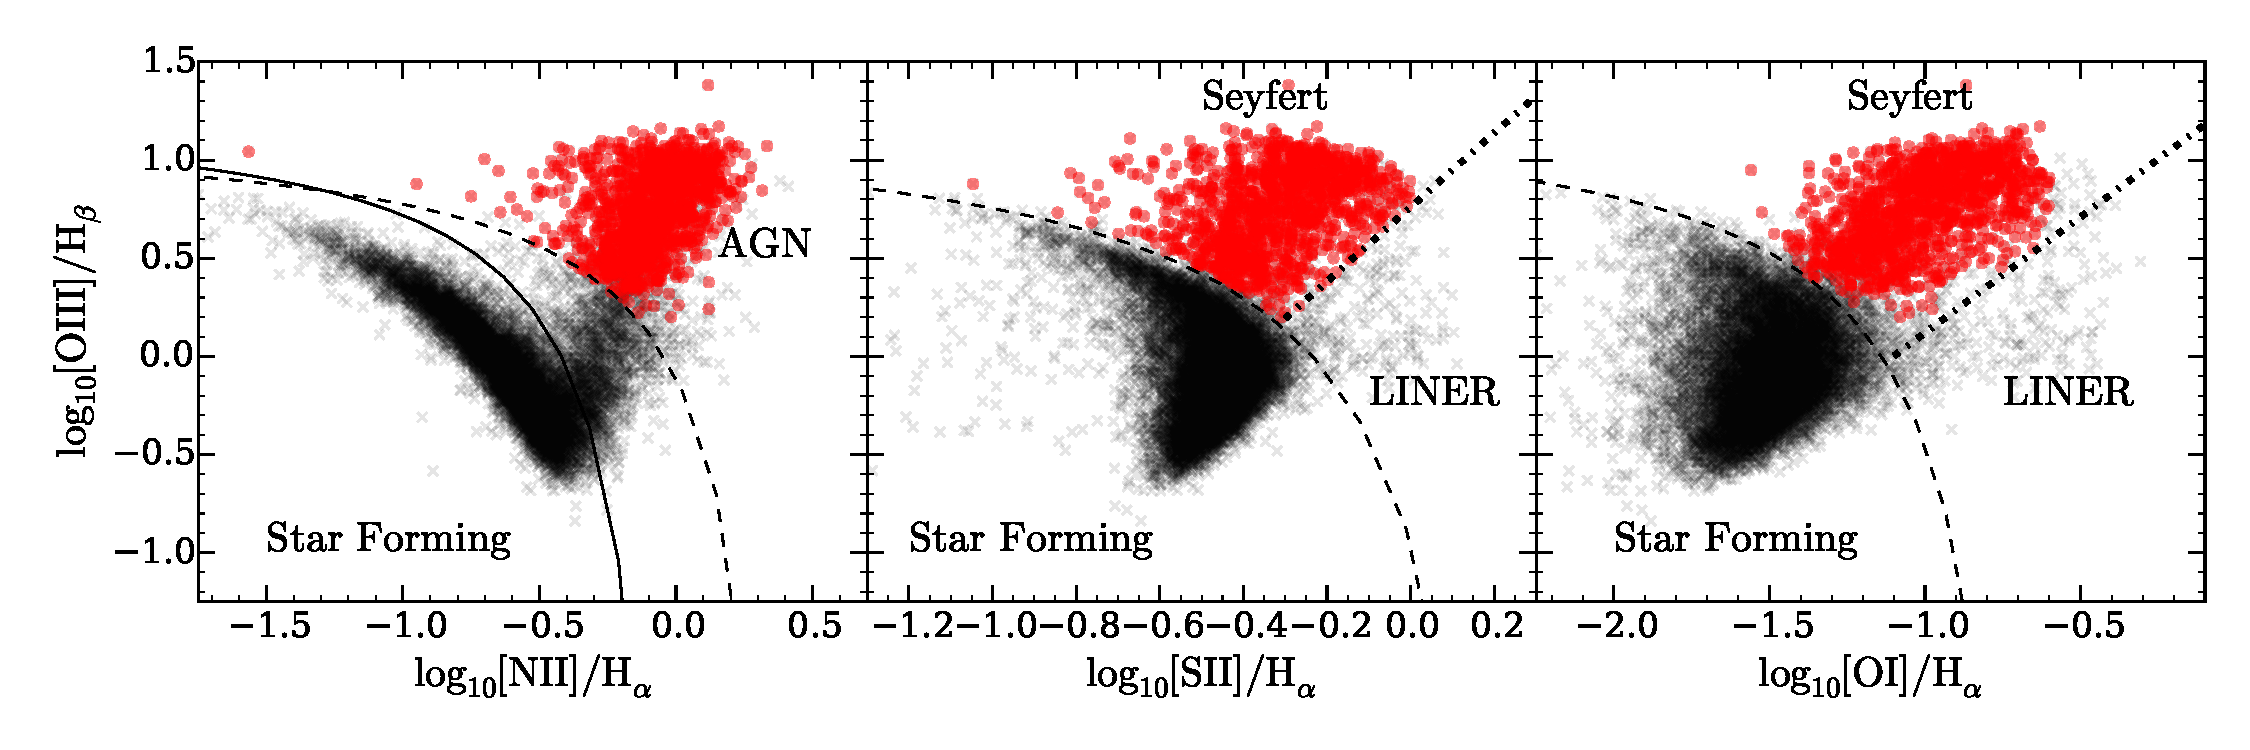
\includegraphics[width=\textwidth]{agn/fig2.pdf}
\caption[BPT diagram used to select AGN host galaxies]{BPT diagrams for galaxies in the \textsc{gz2-galex} sample (black crosses) with S/N $> 3$ for each emission line. Inequalities defined in: \protect\cite{kewley01} to separate SF galaxies from AGN (dashed lines), \protect\cite{kauffmann03b} to separate SF from composite SF-AGN galaxies (solid line) and \protect\cite{kewley06} to separate LINERS and Seyferts (dotted lines). Galaxies are included in the \textsc{agn-host} sample (red circles) if they satisfy all the inequalities to be classified as Seyferts. LINERs are excluded for purity.}
\label{bpt}
\end{figure*}

I do not use Type 1 AGN in this instance due to concerns about contamination of the observed galaxy colours, used in the SFH analysis, from potentially strong NUV emission by unobscured nuclei. The obscuration of Type 2 AGN is highly efficient, considerably more so in the NUV than the optical \citep{Simmons11} so residual NUV flux from a Type 2 AGN can be neglected in comparison to that of the galaxy. I also investigated the possibility of contamination of optical galaxy colours by residual AGN emission and found that subtracting measured nuclear magnitudes (SDSS {\tt psfMag}) produces a negligible change in host galaxy colour ($\Delta(u-r) \sim 0.09$). I therefore use the uncorrected petrosian magnitudes (still with extinction corrections as described in Section~\ref{sec:sample}) to avoid unnecessary complexity and minimise the propagation of uncertainty from the colours through to the inferred SFHs. However, I note that including these corrected colours does not change the results.

Galaxy colours were once again not corrected for intrinsic dust attenuation. This is of particular consequence for disc galaxies, where attenuation increases with increasing inclination. \cite{Buat05} found the median value of the attenuation in the GALEX NUV passband to be $\sim 1$ mag. Similarly \cite{masters10a} found a total extinction from face-on to edge-on spirals of 0.7 and 0.5 mag for the SDSS $u$ and $r$ passbands and show spirals with $\log(a/b) > 0.7$ have signs of significant dust attenuation. For the \textsc{agn-host} (\textsc{inactive}) sample we find $23\%$ ($25\%$) of discs (with $p_d > 0.5$) have $\log(a/b) > 0.7$, therefore we must be aware of possible biases in our results due to dust. 

From the findings of \cite{masters10a} and \cite{Buat05} above, I estimate the extinction to be $u-r \sim 0.2$ mag and $NUV-u \sim 0.3$ mag, therefore the average change in the SFH parameters across a range of input colours $0 ~<~u-r~<~4$ and $-1~<~NUV-u~<~5$,  are $\Delta~t_q~=~0.985$~Gyr, $\Delta~\tau~=~1.571$~Gyr. This change therefore causes the SFH parameters derived to move towards earlier times and faster quenching rates. Results should be viewed with the caveat, particularly for higher mass, disc galaxies, that earlier values of $t_q$ and more rapid values of $\tau$ may be inferred by \textsc{starpy}. However, I note that (i) applying these average corrections across each sample population does not change our main conclusions, (ii) that results are consistent if the population of edge-on and face-on galaxies are compared (see Figure~\ref{dustsplit} and (iii) that results do not change if only face-on galaxies are used in the investigation, strongly suggesting that internal galactic extinction does not systematically bias our results.

Since this investigation is focussed on whether an AGN can have an impact on the SF of its host galaxy, possible selection effects must be considered. The extent to which SF could obscure AGN emission was addressed by \cite{schawinski10a}. They showed, via analysis of simulated AGN emission added to star-forming galaxies, that BPT-based selection of AGN produces a complete sample at luminosities of $L[OIII] > 10^{40}~\rm{erg~s}^{-1}$. Above this limit therefore I assume a complete sample of AGN independent of host galaxy SFR has been selected.

\begin{figure*}
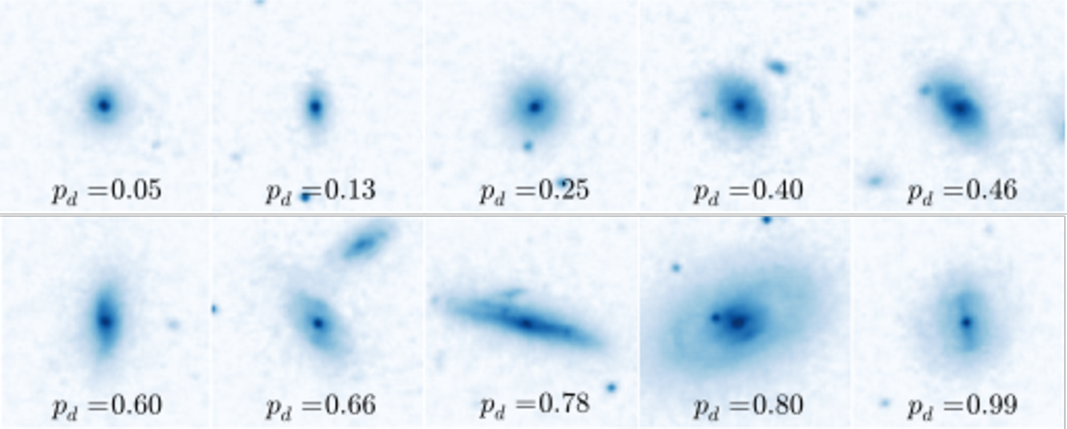
\includegraphics[width=\textwidth]{agn/fig1.pdf}
\caption[SDSS images of galaxies in the \textsc{agn-host} sample]{Randomly selected SDSS \emph{gri} composite images from the sample of $1,244$ Type 2 AGN in a redshift range $0.04 < z < 0.05$.  The galaxies are ordered from least to most featured according to their debiased `disc or featured' vote fraction, $p_d$ (see \citealt{GZ2}). The scale for each image is $0.099~\rm{arcsec/pixel}$.}
\label{mosaic}
\end{figure*}

SDSS images for 10 randomly selected galaxies from the \textsc{agn-host} sample are shown in Figure~\ref{mosaic}.  For the \textsc{agn-host} sample the mean $\log (L[OIII] [\rm{erg~s^{-1}}]) \sim 41.3$ and median $\log (L[OIII] [\rm{erg~s^{-1}}]) \sim 41.0$, with a range of $\log (L[OIII] [\rm{erg~s^{-1}}])$ luminosities of $39.4-43.0$. 


\subsection{Defining a control sample}

A control sample of inactive galaxies was constructed by removing from the \textsc{gz2-galex} sample all galaxies with line strengths indicative of potential AGN activity \citep{kauffmann03b}, as well as sources identified as Type 1 AGN by the presence of broad emission lines \citep{Oh15}.  I selected a mass- and morphology-matched inactive sample by identifying between 1 and 5 inactive galaxies for each \textsc{agn-host} galaxy with the same stellar mass (to within $\pm5\%$) and GZ2 `smooth' and `disc' vote fractions (to within $\pm 0.1$) giving $6107$ galaxies. This sample will be referred to as the \textsc{inactive} sample. A Kolmogorov-Smirnov test revealed the redshift distributions of the \textsc{inactive} and \textsc{agn-host} samples are statistically indistinguishable ($D \sim 0.16$, $p \sim 0.88$). 

The \textsc{agn-host} and \textsc{inactive}  samples are shown on both an optical colour-magnitude diagram and in the SFR-stellar mass plane in Figure~\ref{cmdsfms} in comparison to the distribution of SDSS DR7 galaxies. SFRs and stellar masses are obtained from the MPA JHU catalog, where available, which follow the prescriptions outlined in \cite{brinchmann04} and \cite{Salim07} for calculating the total aperture corrected galaxy SFR in the presence of an AGN. 

The majority of the \textsc{agn-host} sample would be defined as residing in the blue cloud ($73\%$) on the optical colour-magnitude diagram despite the fact that a significant proportion of the sample ($47\%$) lie more than $1\sigma$ ($0.3$ $\rm{dex}$) below the star forming ``main sequence'' (fit to the MPA-JHU catalog of SDSS DR7 of \citealt{kauffmann03, brinchmann04}, see Figure \ref{cmdsfms}). I do not make a cut on either the \textsc{agn-host} or \textsc{inactive} samples for star formation rate. The SFH of the entire samples are fitted, however I describe in Section \ref{popstarpy} how the \textsc{popstarpy} method accounts for those galaxies not appropriately fit by a quenching model and down-weights their contribution to the final results.

\begin{figure}
\centering
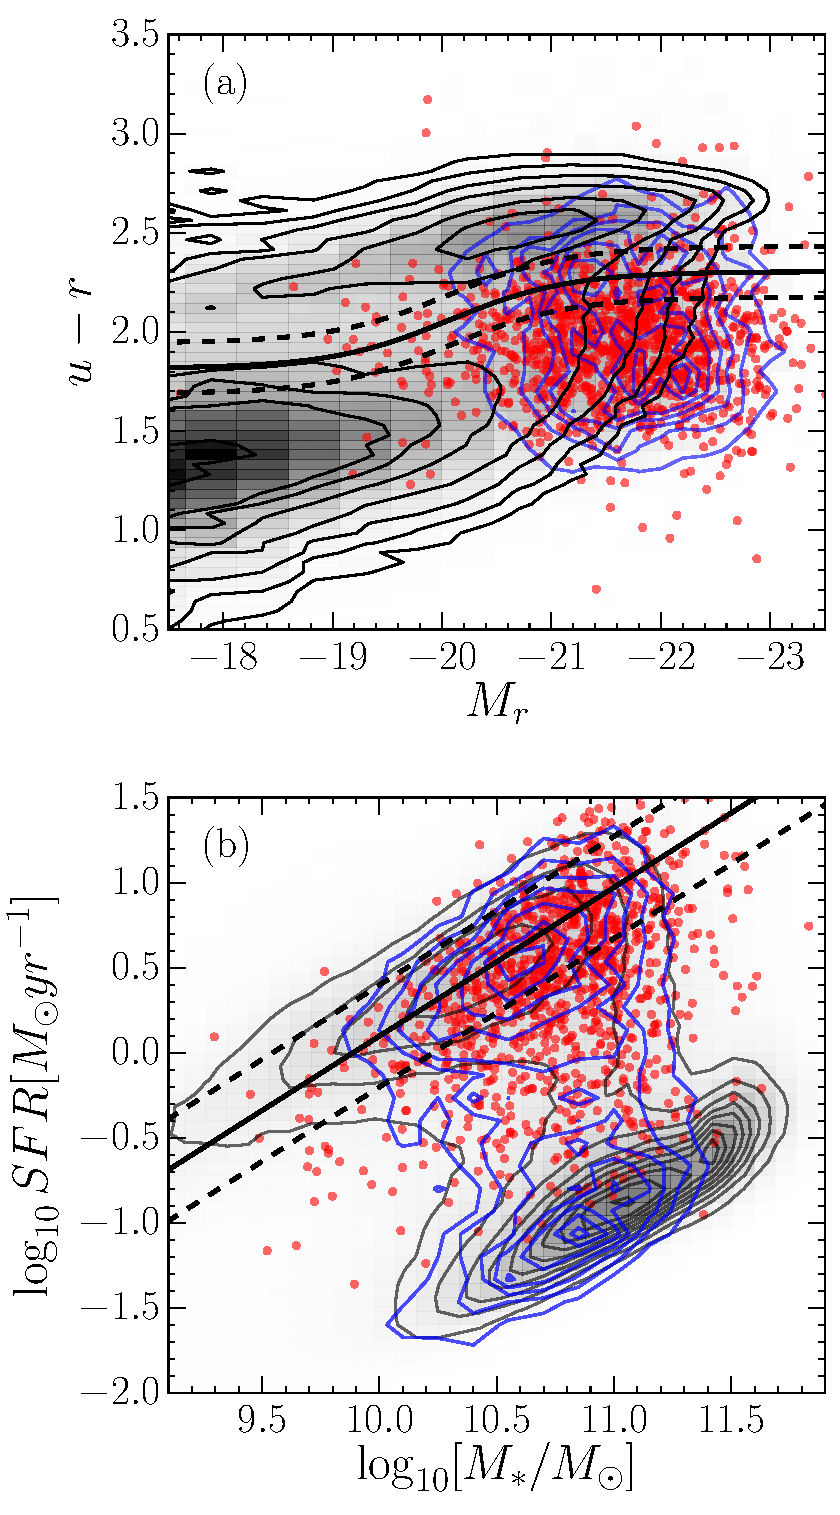
\includegraphics[height=0.75\textheight]{agn/fig3.pdf}
\caption[Colour-magnitude and SFR-mass diagram for \textsc{agn-host} galaxies]{(a) Optical colour-magnitude diagram showing the SDSS DR7 (grey filled contours), the \textsc{agn-host} sample (red circles) and \textsc{inactive} sample (blue contours). The definition of the green valley from \citet{Baldry06} (solid line) with $\pm 1\sigma$ (dashed lines) is shown. (b) SFR-stellar mass diagram showing the MPA-JHU measurements of SFR and $M_*$ of SDSS DR7 galaxies (\citealt{kauffmann03, brinchmann04}; black contours), the \textsc{agn-host} sample (red circles) and \textsc{inactive} sample (blue contours). The star forming ``main sequence'' from \citet{peng10} is shown by the solid line for $t = 12.8~\rm{Gyr}$, the average observed age of the \textsc{gz2-galex} sample, with $\pm1\sigma$ (dashed lines).}
\label{cmdsfms}
\end{figure}

\subsection{Results}\label{results}

\begin{figure*}
\centering{
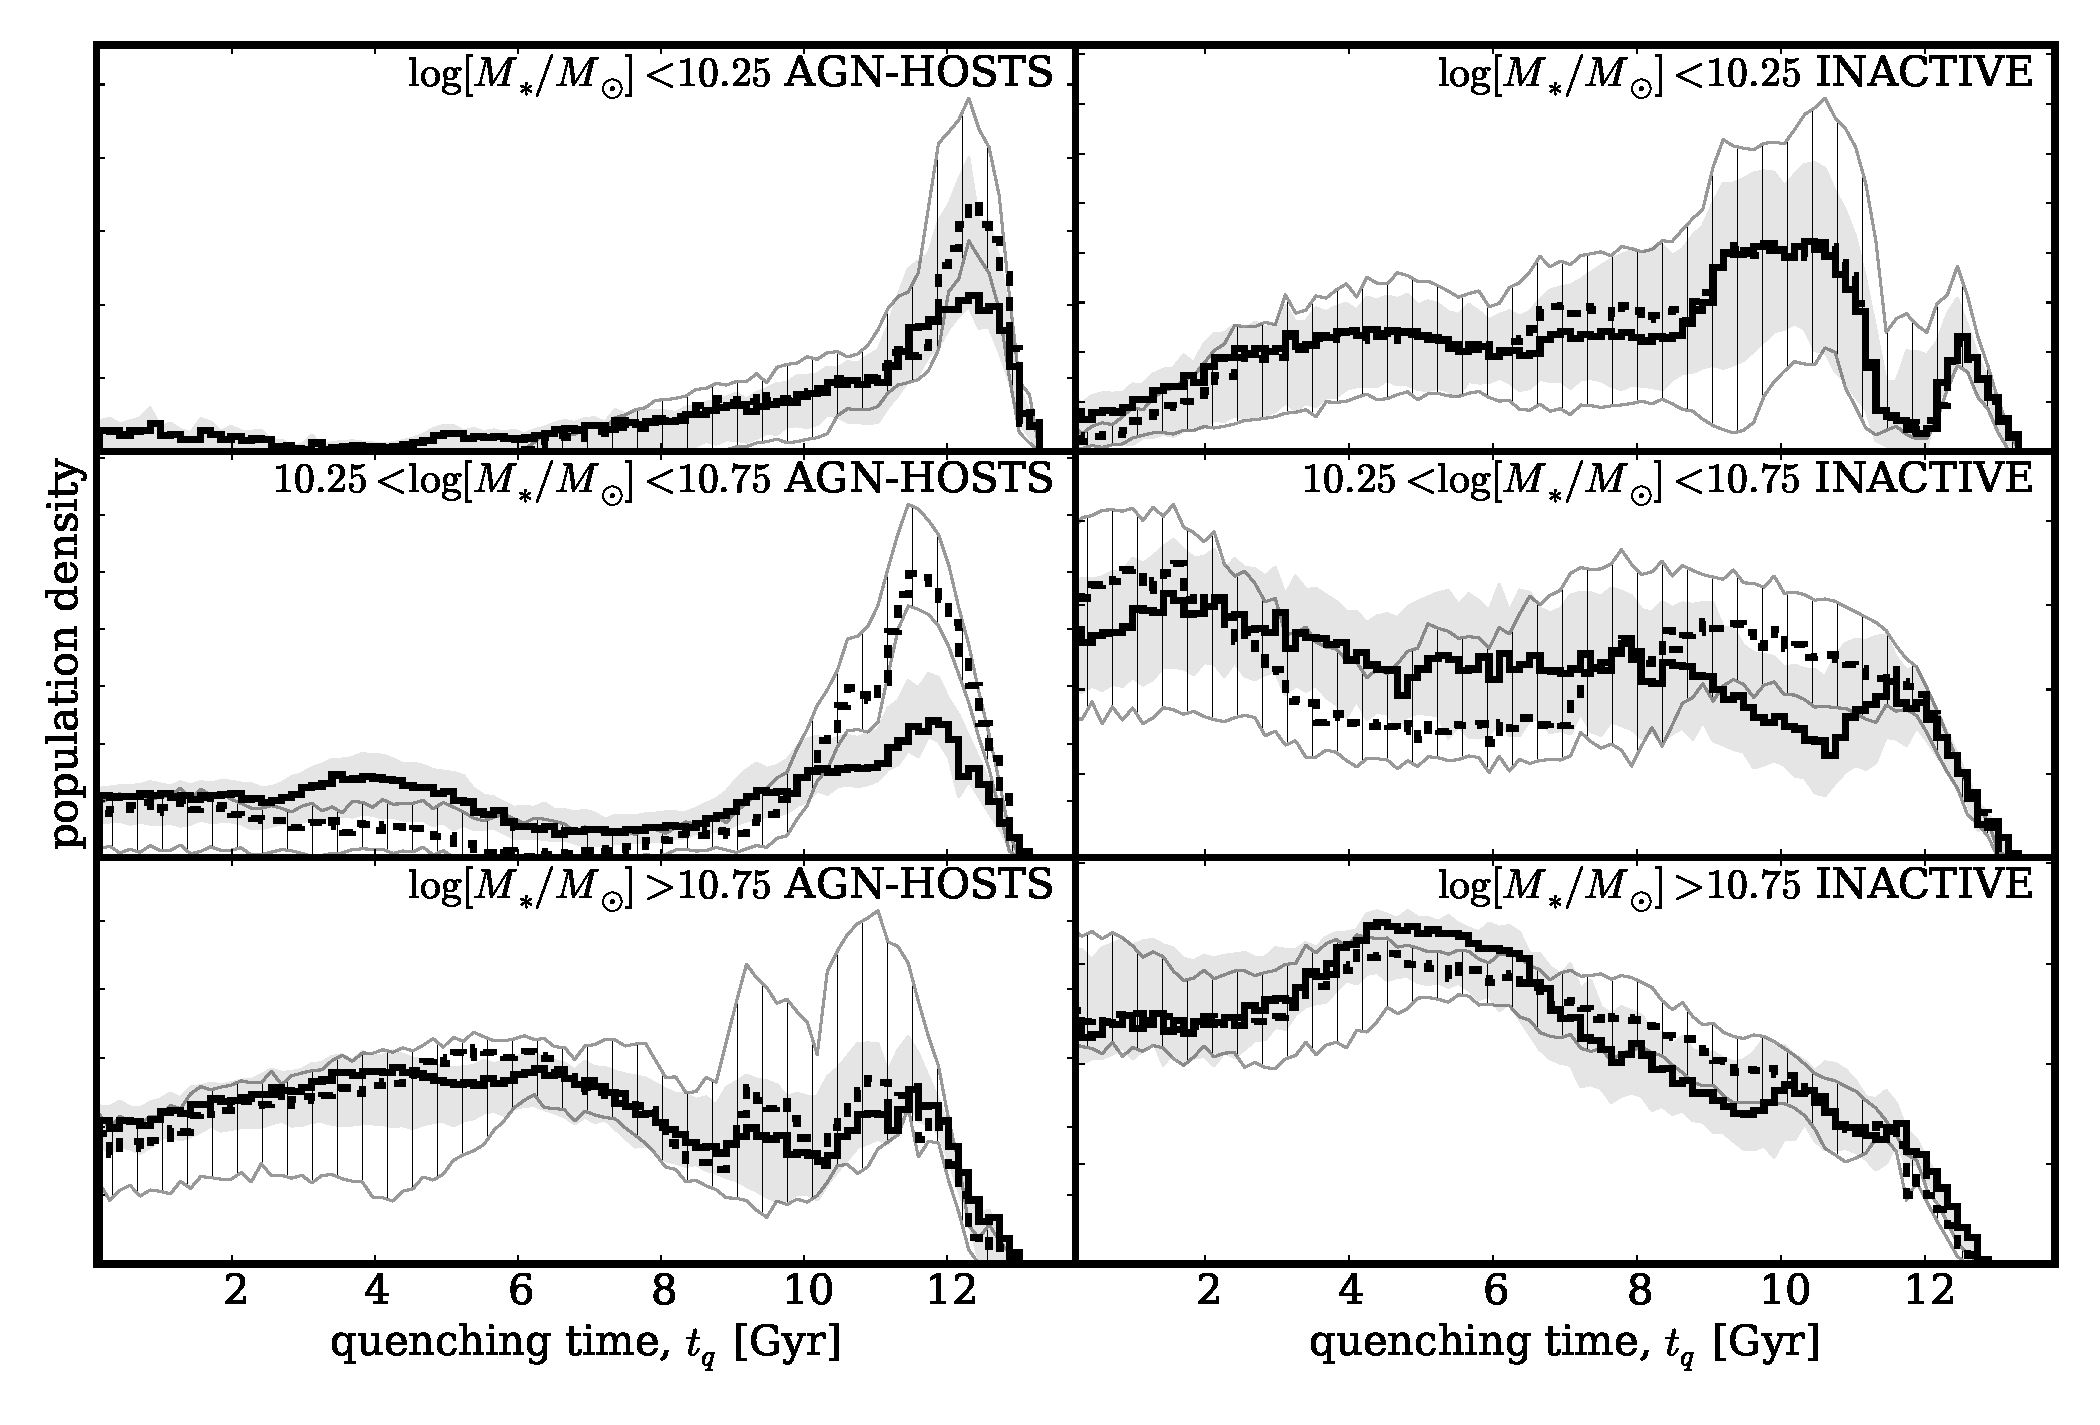
\includegraphics[width=0.92\textwidth]{agn/fig4.pdf}}
\caption[Quenching time population density distributions for the \textsc{agn-host} and \textsc{inactive} samples] {Population density distributions for the quenching time ($t_q$) parameter, normalised so that the areas under the curves are equal. \textsc{agn-host} (left) and \textsc{inactive} (right) galaxies are split into low (top), medium (middle) and high (bottom) mass for smooth (dashed) and disc (solid) galaxies. Uncertainties from bootstrapping are shown by the shaded regions for the smooth (grey striped) and disc (grey solid) population densities. A low (high) value of $t_q$ corresponds to the early (recent) Universe.}
\label{time}
\end{figure*}


\begin{figure*}
\centering{
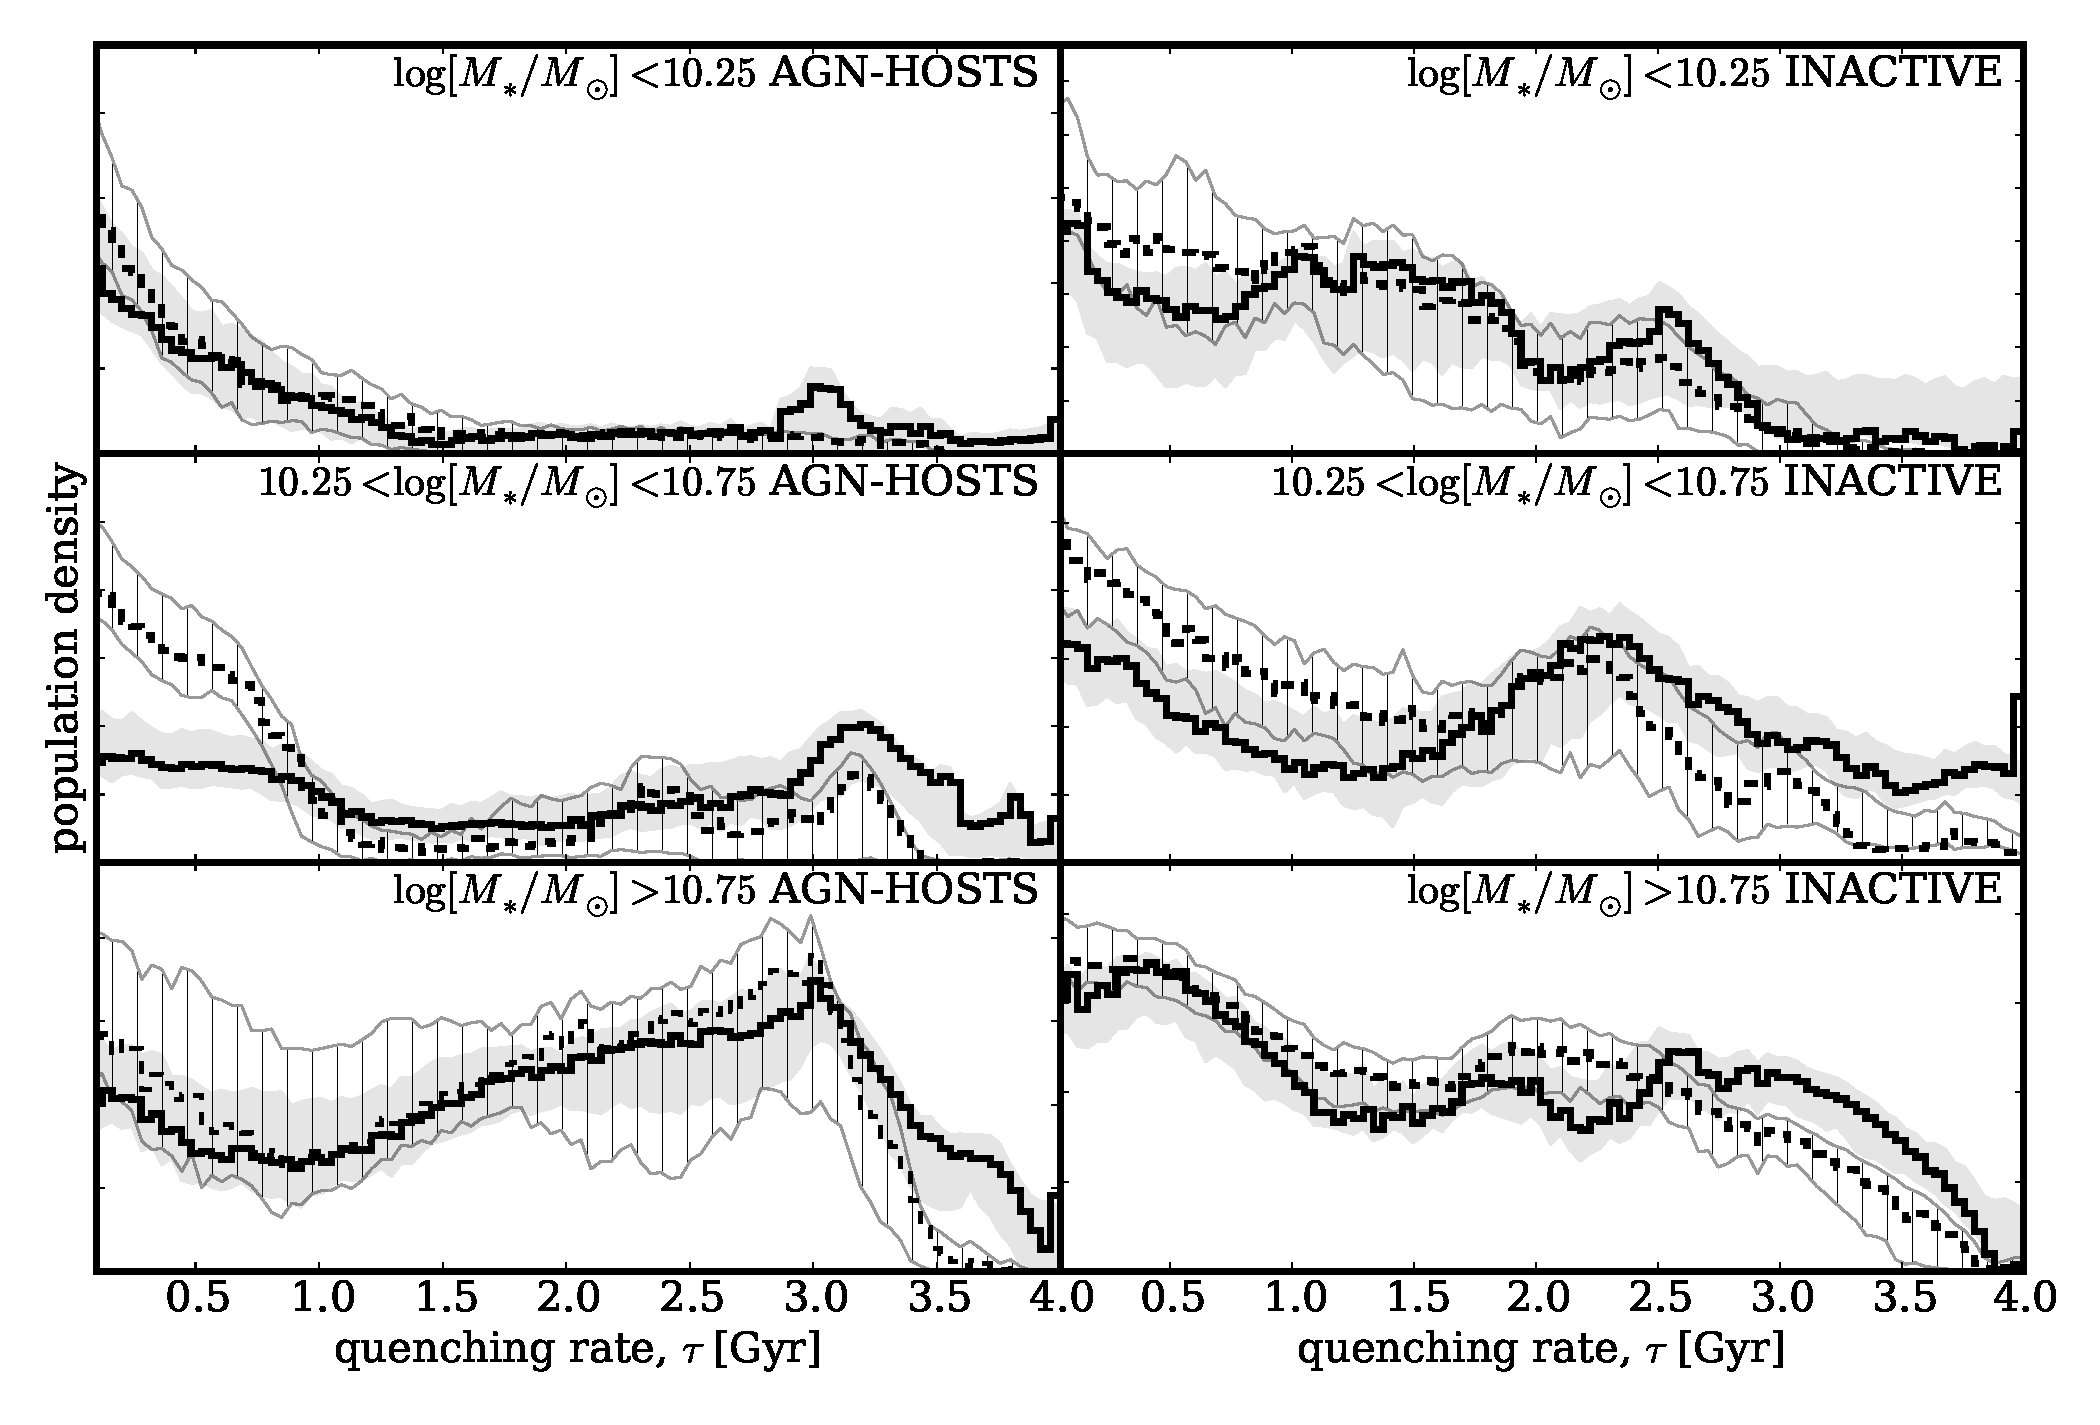
\includegraphics[width=0.92\textwidth]{agn/fig5.pdf}}
\caption[Quenching rate population density distributions for the \textsc{agn-host} and \textsc{inactive} samples]{Population density distributions for the quenching rate ($\tau$), normalised so that the areas under the curves are equal. \textsc{agn-host} (left) host and \textsc{inactive} (right) galaxies are split into low (top), medium (middle) and high (bottom) mass for smooth (dashed) and disc (solid) galaxies. Uncertainties from bootstrapping are shown by the shaded regions for the smooth (grey striped) and disc (grey solid) population densities. A small (large) value of $\tau$ corresponds to a rapid (slow) quench.}
\label{rate}
\end{figure*}

Figures~\ref{time} and \ref{rate} show the stacked population density distributions for the quenching time, $t_q$ and exponential quenching rate, $\tau$, respectively. In each figure the population density, along with shaded regions to show the uncertainties, for a given parameter is shown for smooth and disc galaxy populations across three mass bins for the \textsc{agn-host} and \textsc{inactive} samples. No cut on the star formation rate is made to the galaxies which contribute to Figures \ref{time} \& \ref{rate}, but those galaxies poorly fit by an exponentially declining SFH are down-weighted so that they do not contribute to the results presented here. In Table~\ref{massbins} the percentage of the  population density in each quenching regime for rapid ($\tau < 1$ Gyr), intermediate ($1 < \tau ~\rm{[Gyr]} < 2$) and slow ($\tau > 2$ Gyr) quenching timescales, are shown. Uncertainties on the population densities (shown by the shaded regions) are determined from the maximum and minimum values spanned by $N = 1000$ bootstrap iterations, each sampling $90\%$ of the galaxy population. $1\sigma$ uncertainties are quoted for the percentages in Table~\ref{massbins}, calculated from the bootstrapped distributions.


\begin{table*}
{\tiny
\centering{
\caption{Table showing the number of galaxies in each of the three mass bins for both the \textsc{agn-hosts} and \textsc{inactive} galaxy samples and the percentage of the distribution across each morphologically weighted population found in the rapid, intermediate and slow quenching regimes.}
\label{massbins}
\begin{tabular}{c|c|c|c|c|c|c}
\hline
\textsc{sample}                     & \textsc{mass bin}                                        & \textsc{weighting}                  & $\tau < 1 ~\rm{[Gyr]}$                             & $1 < \tau ~\rm{[Gyr]} < 2 $          & $\tau > 2 ~\rm{[Gyr]}$                               & \textsc{number}                                        \\ \hline \hline
\multirow{6}{*}{AGN-HOSTS} & \multirow{2}{*}{$\log [M_*/M_{\odot}] < 10.25 $}                       & $p_d$     & $60\pm_{5}^{23}$                    & $13\pm_{9}^{9}$                    & $28\pm_{19}^{6}$       & \multirow{2}{*}{$165 (13.3\%)$}                      \\
                           &                                                 & $p_s$     & $69\pm_{6}^{14}$                    & $17\pm_{14}^{6}$                   & $14\pm_{7}^{3}$        &                                                      \\ \cline{2-7} 
                           & \multirow{2}{*}{$10.25 < \log [M_*/M_{\odot}] < 10.75$}                    & $p_d$     & $33\pm_{5}^{3}$                     & $15\pm_{4}^{4}$                    & $51\pm_{7}^{4}$        & \multirow{2}{*}{$630 (50.6\%)$}                      \\
                           &                                                 & $p_s$     & $69\pm_{5}^{4}$                     & $7\pm_{4}^{4}$                     & $26\pm_{9}^{5}$        &                                                      \\ \cline{2-7} 
                           & \multirow{2}{*}{$\log [M_*/M_{\odot}] > 10.75$}                      & $p_d$     & $20\pm_{4}^{5}$ & $25\pm_{5}^{7}$                    & $56\pm_{12}^{8}$       & \multirow{2}{*}{$449 (36.1\%)$}                      \\
                           &                                                 & $p_s$     & $24\pm_{3}^{4}$                     & $26\pm_{6}^{5}$                    & $50\pm_{7}^{7}$        &                                                      \\ \hline \hline
\multirow{6}{*}{INACTIVE}  & \multirow{2}{*}{$\log [M_*/M_{\odot}] < 10.25 $}                       & $p_d$     & $37\pm_{14}^{8}$                    & $39\pm_{6}^{8}$                    & $24\pm_{6}^{8}$        & \multirow{2}{*}{$807 (13.2\%)$}                      \\
                           &                                                 & $p_s$     & $47\pm_{11}^{5}$                    & $36\pm_{5}^{9}$                    & $17\pm_{5}^{4}$        &                                                      \\ \cline{2-7} 
                           & \multirow{2}{*}{$10.25 < \log [M_*/M_{\odot}] < 10.75$}                    & $p_d$     &          $30\pm_{3}^{4}$                          &       $18\pm_{3}^{2}$                            &    $51\pm_{4}^{4}$                   & \multirow{2}{*}{$3094 (50.7\%)$}                     \\
                           &                                                 & $p_s$     & $42\pm_{2}^{2}$            & $29\pm_{3}^{3}$   & $30\pm_{4}^{3}$ &                                                      \\ \cline{2-7} 
                           & {\multirow{2}{*}{$\log [M_*/M_{\odot}] > 10.75$}} & $p_d$     & $36\pm_{3}^{3}$            & $24\pm_{4}^{3}$         & $41\pm_{3}^{4}$ & \multicolumn{1}{l}{\multirow{2}{*}{$2206 (36.1\%)$}} \\
                           & \multicolumn{1}{l|}{}                           & $p_s$      & $38\pm_{2}^{2}$              & $28\pm_{4}^{3}$            & $34\pm_{3}^{3}$ & \multicolumn{1}{l}{}                                 \\ \hline                       
\end{tabular}}}
\end{table*}

These population densities should be interpreted as the spread of quenching times and rates occurring in galaxies which have either undergone or are undergoing quenching within a population. Figures~\ref{time} and \ref{rate} show a distinct difference between the population density of \textsc{agn-host} and \textsc{inactive} quenching parameters.

At all masses, the population density for galaxies within the \textsc{agn-host} population across the quenching time $t_q$ parameter (left panels of Figure~\ref{time}) is different from that of the inactive galaxies (right panels of Figure~\ref{time}). Recent quenching ($t > 11$ Gyr) is the dominant history for quenched and quenching low and medium mass \textsc{agn-host} galaxies, particularly for the smooth galaxies hosting an AGN. However, this effect is less dominant in higher mass galaxies where quenching at earlier times also has high density.


The population densities for the quenching rate, $\tau$, in Figure~\ref{rate} and Table~\ref{massbins} show the dominance of rapid quenching ($\tau < 1$ Gyr) within the \textsc{agn-host} population, particularly for smooth galaxies. With increasing mass the dominant quenching rate becomes slow ($\tau > 2$ Gyr) especially for disc galaxies hosting an AGN. Similar trends in the density are observed within the \textsc{inactive} population but the overall distribution is very different. 


The distributions for the \textsc{agn-host} galaxies therefore show evidence for the dominance of rapid, recent quenching within this population. This result implies the importance of AGN feedback for the evolution of these galaxies.

\subsection{Discussion}\label{dis}

The differences between the population density distributions of the \textsc{agn-host} and \textsc{inactive} populations reveal that an AGN can have a significant effect on the SFH of its host galaxy. Both recent, rapid quenching and early, slow quenching are observed in the population density of the \textsc{agn-host} population. 


There are minimal differences between the smooth and disc weighted distributions of the quenching parameters within the \textsc{agn-host} population. This is agreement with the conclusions of \citet{kauffmann03b} who found that the structural properties of AGN hosts depend very little on AGN power. The AGN therefore do not care about the morphology of their host galaxies. 


The difference between the \textsc{agn-host} and \textsc{inactive} population distributions in Figure~\ref{rate} for the rate of quenching, $\tau$, tells a story of gas reservoirs. The density distribution for higher mass \textsc{agn-host} galaxies is dominated by slow, early quenching implying another mechanism is responsible for the cessation of star formation within a proportion of these high mass galaxies prior to the triggering of the current AGN.  This preference for slow evolution timescales follows from the ideas of previously isolated discs evolving slowly by the Kennicutt-Schmidt \citep{Schmidt59, Kennicutt97} law which can then undergo an interaction or merger to reinvigorate star formation, feed the central black hole and trigger an AGN \citep{Varela04, emsellem15}. These galaxies would need a large enough gas reservoir to fuel both SF throughout their lifetimes and the recent AGN. These high mass galaxies also play host to the most luminous AGN (mean $\log (L[OIII] ~[\rm{erg}~s^{-1}]) \sim 41.6$) and so this SFH challenges the usual explanation for the co-evolution of luminous black holes and their host galaxies driven by merger growth (see Section~\ref{intbulgeless} for an investigation into an alternative merger free black hole-galaxy co-evolution). 


Quenching at early times is also observed within a subsample of the \textsc{inactive} population, where the density for the quenching time is roughly constant until recent times where the distribution drops off.  This drop-off occurs at earlier times with increasing mass with a significant lack of quenching occurring at early times for low mass \textsc{inactive} galaxies (right panels Figure~\ref{time}). This is evidence of downsizing within the \textsc{inactive} galaxy population whereby stars in massive galaxies form first and quench early \citep{Cowie96, Thomas10}. 

Some of the most massive \textsc{agn-host} galaxies also show a preference for earlier quenching (bottom left panel Figure~\ref{time}) occurring at slow rates; I speculate that this is also due to the effects of downsizing rather than being caused by the current AGN. This earlier evolution would first form a slowly `dying' or `dead' galaxy typical of massive elliptical galaxies which can then have a recent infall of gas either through a minor merger, galaxy interaction or environmental change, triggering further star formation and feeding the central black hole, triggering an AGN \citep{kaviraj14b}. In turn this AGN can then quench the recent boost in star formation. This track is similar to the evolution history proposed for blue ellipticals \citep{Kaviraj13, McIntosh14, Haines15}. This SFH would then give rise to the distribution seen within the high mass \textsc{agn-host} population for both time and rate parameters.


These recently triggered AGN in both massive disc and smooth galaxies do not have have the ability to impact the SF across the entirety of a high mass galaxy in a deep gravitational potential \citep{ishibashi12, Zinn13}. This leads to the lower peak for recent, rapid quenching within the high mass \textsc{agn-host} population for both morphologies. 

Conversely, rapid quenching, possibly caused by the AGN itself through negative feedback, is the most dominant history within the low mass \textsc{agn-host} population with lower gravitational potentials from which gas may be more readily expelled or heated \citep{tortora09}. 

\cite{tortora09} model the effects of jet-induced AGN feedback on a typical early type (i.e. smooth) galaxy and observe a drastic suppression of star formation on a timescale of $\sim 3 ~\rm{Myr}$. Comparing their synthetic colours with observed colours of SDSS elliptical galaxies, they find the time between the current galaxy age, $t_\mathrm{gal}$ and the time that the feedback began, $t_\mathrm{AGN}$, peaks at $t_\mathrm{gal} - t_\mathrm{AGN} \sim 0.85 ~\rm{Gyr}$. This agrees with the location of the peak in Figure~\ref{time} for low mass galaxies  which have undergone quenching, where the difference between the peak of the distribution and the average age of the population (galaxy age is calculated as the age of the Universe at the observed redshift, by assuming all galaxies form at $t=0$) is $\sim0.83 ~\rm{Gyr}$. This implies that this SFH dominated by recent quenching is caused directly by negative AGN feedback.


However, there still remains the possibility that the AGN is merely a consequence of an alternative quenching mechanism. This idea is supported by simulations showing that the exhaustion of gas by a merger fuelled starburst could cause such a rapid quench in star formation and in turn also trigger an AGN \citep{Croton06, Wild09, Snyder11, Hayward14}. \citet{Yesuf14} also showed that AGN are more commonly hosted by post starburst galaxies, with the peak AGN activity appearing $\geq 200 \pm 100 ~\rm{Myr}$ after the starburst. Such a SFH is not accounted for in the models presented here (see Section ~\ref{future} for a discussion), however this scenario is still consistent with the results presented in this paper; that AGN which are \emph{currently} active have been detected in host galaxies $\sim 1~\rm{Gyr}$ after the onset of quenching.

This rapid quenching is particularly dominant for low-to-medium mass smooth galaxies. \cite{smethurst15} suggest that incredibly rapid quenching rates could be attributed to mergers of galaxies in conjunction with AGN feedback, which are thought to be responsible for creating the most massive smooth galaxies \citep{conselice03b, springel05b, hopkins08b}. This dominance of rapid quenching across the smooth \textsc{agn-host} population supports the idea that a merger, having caused a morphological transformation to a smooth galaxy, can also trigger an AGN, causing feedback and cessation of star formation (\citealt{Sanders88, pontzen16}).

Within the medium mass \textsc{agn-host} population we see a bimodal distribution between these two quenching histories, highlighting the strength of this method which is capable of detecting such variation in the SFHs within a population of galaxies. 

Indeed not all galaxies in the \textsc{agn-host} and \textsc{inactive} samples are quenching, as seen in Figure \ref{cmdsfms}, with a significant proportion of both the \textsc{agn-host} and \textsc{inactive} samples lying on the star forming sequence. A galaxy can therefore still maintain star formation whilst hosting an AGN. The results presented in Section \ref{results} only reflect the trends for galaxies that have undergone or are currently undergoing quenching within a population and can therefore be accurately fit by an exponentially declining SFH. This prevalence of star forming AGN host galaxies, combined with the results above allows us to consider that either: (i)  the AGN are the cause of the rapid quenching observed but only in gas-poor host galaxies where they can have a large impact, (ii) the AGN are a consequence of another quenching mechanism but can also be triggered by other means which do not cause quenching, or (iii) the SFR of a galaxy can recover post-quench and return to the star forming sequence after a few Gyr (see recent simulations by \citealt{pontzen16}). Further investigation will therefore be required to determine the nature of this quenching (see Section \ref{future} for a discussion of the future work).

%INSERT PARAGRAPH ON HOW TIES IN WITH LUMINOSITY FUNCTION 

\newpage

\section{Bulgeless galaxies hosting growing black holes}\label{intbulgeless}

\emph{The work in the following chapter has been submitted to MNRAS in Simmons, Smethurst \& Lintott (subm.). I was responsible for the data reduction, statistical analysis and assisted in the interpretation of the results.}

%INSERT PARAGRAPH LEADING ON FROM PREVIOUS SECTION
In Section \ref{agnfeedback}, I showed how disc galaxies currently hosting an AGN could have started quenching at early times with very slow quenching timescales. This secular co-evolution of the galaxy and black hole has been proposed before and investigated by \citet{Simmons13} with AGn residing in disk dominated hosts whose accretion histories are assumed to be merger free. In the following work we investigate a larger sample of disc galaxies identified as bulgeless or disk dominated with an AGN and measure their black hole masses. 

%%%%%%%%%%%%%%%%%%%%%%%%%%%%%%%%%%%%%%%%%%%%%%
%
%
\subsection{Observational Data}\label{sec:data}
%
%
%%%%%%%%%%%%%%%%%%%%%%%%%%%%%%%%%%%%%%%%%%%%%%

The goal of this study is to investigate black hole growth in galaxies whose growth histories have been dominated by relatively calm processes. We therefore require a sample of growing black holes hosted in disk-dominated galaxies. Optimally, the AGN should have broad emission lines to facilitate measurement of black hole masses via well-established relations between line flux and width and black hole masses. Previously, \citet{simmons13} investigated a sample of 13 pure disk galaxies hosting AGN. The selection method used in that study selected against very massive black holes with unobscured emission: only 2 AGN of 13 show clear signs of broadened line emission in their SDSS spectra, with masses of $4 \times 10^6$ and $1 \times 10^7 \mmsun $. Here we aim to select AGN at all masses but with broad emission lines, and which are hosted in disk-dominated galaxies. Below we describe the method used to select this sample and the data sets from which the sample is drawn.

%%%%%%%%%%%%%%%%%%%%%%%%%%%%%%%%%%%%%%%%%%%%%%
\subsubsection{AGN Selection}
% including where we get AGN luminosities from
%%%%%%%%%%%%%%%%%%%%%%%%%%%%%%%%%%%%%%%%%%%%%%

Examining the black hole-galaxy relation requires selection of a sample of unobscured AGN with broad emission lines, so that black hole masses may be measured from well-established correlations between emission line properties and black hole masses {\notebsm \citep[e.g.,][]{jiang11a,xiao11}}. 

Unobscured AGN have characteristic colours in multi-wavelength imaging, particularly in X-ray, optical and infrared bands \citep{sdss_qso_color_selection,xray_agn_selection,ir_agn_selection}. Given the existence of all-sky surveys at many of the wavelengths relevant to the selection of unobscured AGN, it is now possible to construct samples of sources identified as unobscured AGN with high likelihood.

We select an initial sample of AGN using the W2R sample of \citet{edelson12}, comprised of 4316 sources identified using multi-wavelength data from the \emph{Wide-field Infrared Survey Explorer} \citep[\emph{WISE};][]{wright10}, Two Micron All-Sky Survey \citep[2MASS;][]{skrutskie06}, and \emph{ROSAT} all-sky survey \citep[RASS;][]{voges99}. This is a photometric, all-sky selection, which selects unobscured AGN at $>95$ per cent confidence \citet{edelson12}.



%%%%%%%%%%%%%%%%%%%%%%%%%%%%%%%%%%%%%%%%%%%%%%
\subsubsection{Selecting disk-dominated AGN host galaxies}
% including source of optical imagery
%%%%%%%%%%%%%%%%%%%%%%%%%%%%%%%%%%%%%%%%%%%%%%



\begin{figure*}
\centering{
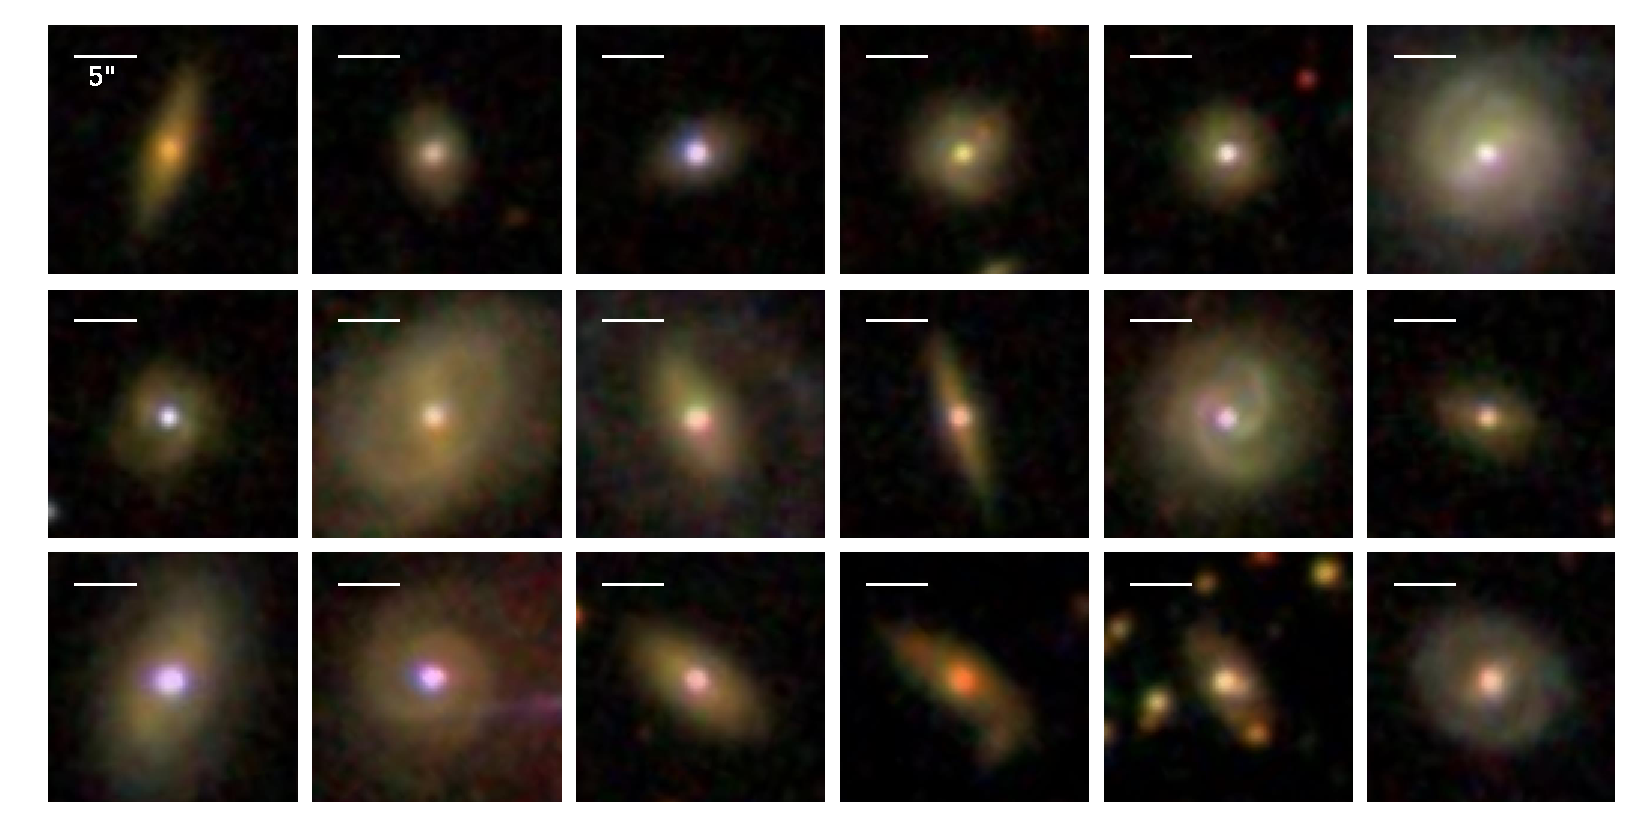
\includegraphics[width=\textwidth]{agn/mosaic_random_13_int5.pdf}
\caption[SDSS images of selected bulgeless, disc dominated galaxies]{Example postage stamp SDSS images of galaxies within the sample of 101 bulgeless galaxies for which we have spectra. The last 5 images on the bottom row are the galaxies observed with the IDS on the INT. The scale for each image is shown by the $5^{\prime \prime}$ ruler in each panel.  
}}
\label{fig:exampleimages}
\end{figure*}


Following the AGN selection described above, we further sub-select galaxies imaged by the Sloan Digital Sky Survey. There are 1,844 W2R sources with positional matches having reported coordinates within $3^{\prime \prime}$ of a source in SDSS \citep{york00} Data Release 8 \citep{sdssdr8}, a fraction consistent with the fractional area of the SDSS versus an all-sky catalog. 76 per cent of this sub-sample has measured redshifts, with a peak redshift distribution of $z \approx 0.12$.  90 percent of sources with redshifts have $z < 0.6$; the distribution has a long tail to $z_{\rm max} = 2.35$.

We then examine each SDSS colour cutout to identify disk-dominated features. One author (BDS) identified ??? (SDSS+13+INTB) disk-dominated AGN host galaxies on the basis of clearly identifiable spiral arms, bars or obvious edge-on disks. Figure \ref{fig:exampleimages} shows a sample of these galaxies.



%%%%%%%%%%%%%%%%%%%%%%%%%%%%%%%%%%%%%%%%%%%%%%
\subsubsection{Spectra}\label{sec:spectra}
%%%%%%%%%%%%%%%%%%%%%%%%%%%%%%%%%%%%%%%%%%%%%%

Of the ??? disk-dominated AGN host galaxies with SDSS imaging observations, 73 have spectra from SDSS Data Release 9 \citep{dr9_ref}. The others are not included because they lie outside the Data Release 7 footprint (which had high spectral completeness) and were not targets for any SDSS-III projects (which have specific requirements and generally do not include AGN host galaxies with low enough redshift to identify spiral arms in SDSS imaging). {\notebsm 23 also have spectra and were identified from Chen and Edelson \& Malken.}  We measured the broad $H\alpha$ emission for  {\notebsm 5 additional sources} using long-slit spectra using IDS on INT from 21st-23rd May 2014. Spectra were reduced using the standard reduction pipeline of Massey, Valdes \& Barnes (1992) using IRAF modules to debiased, dark subtract, flat field, calibrate, sky subtract, flux calibrate and extract spectra. These reduced spectra are shown in Figure \ref{fig:INTspectra} for the 5 galaxies observed.


\begin{figure*}
\centering{
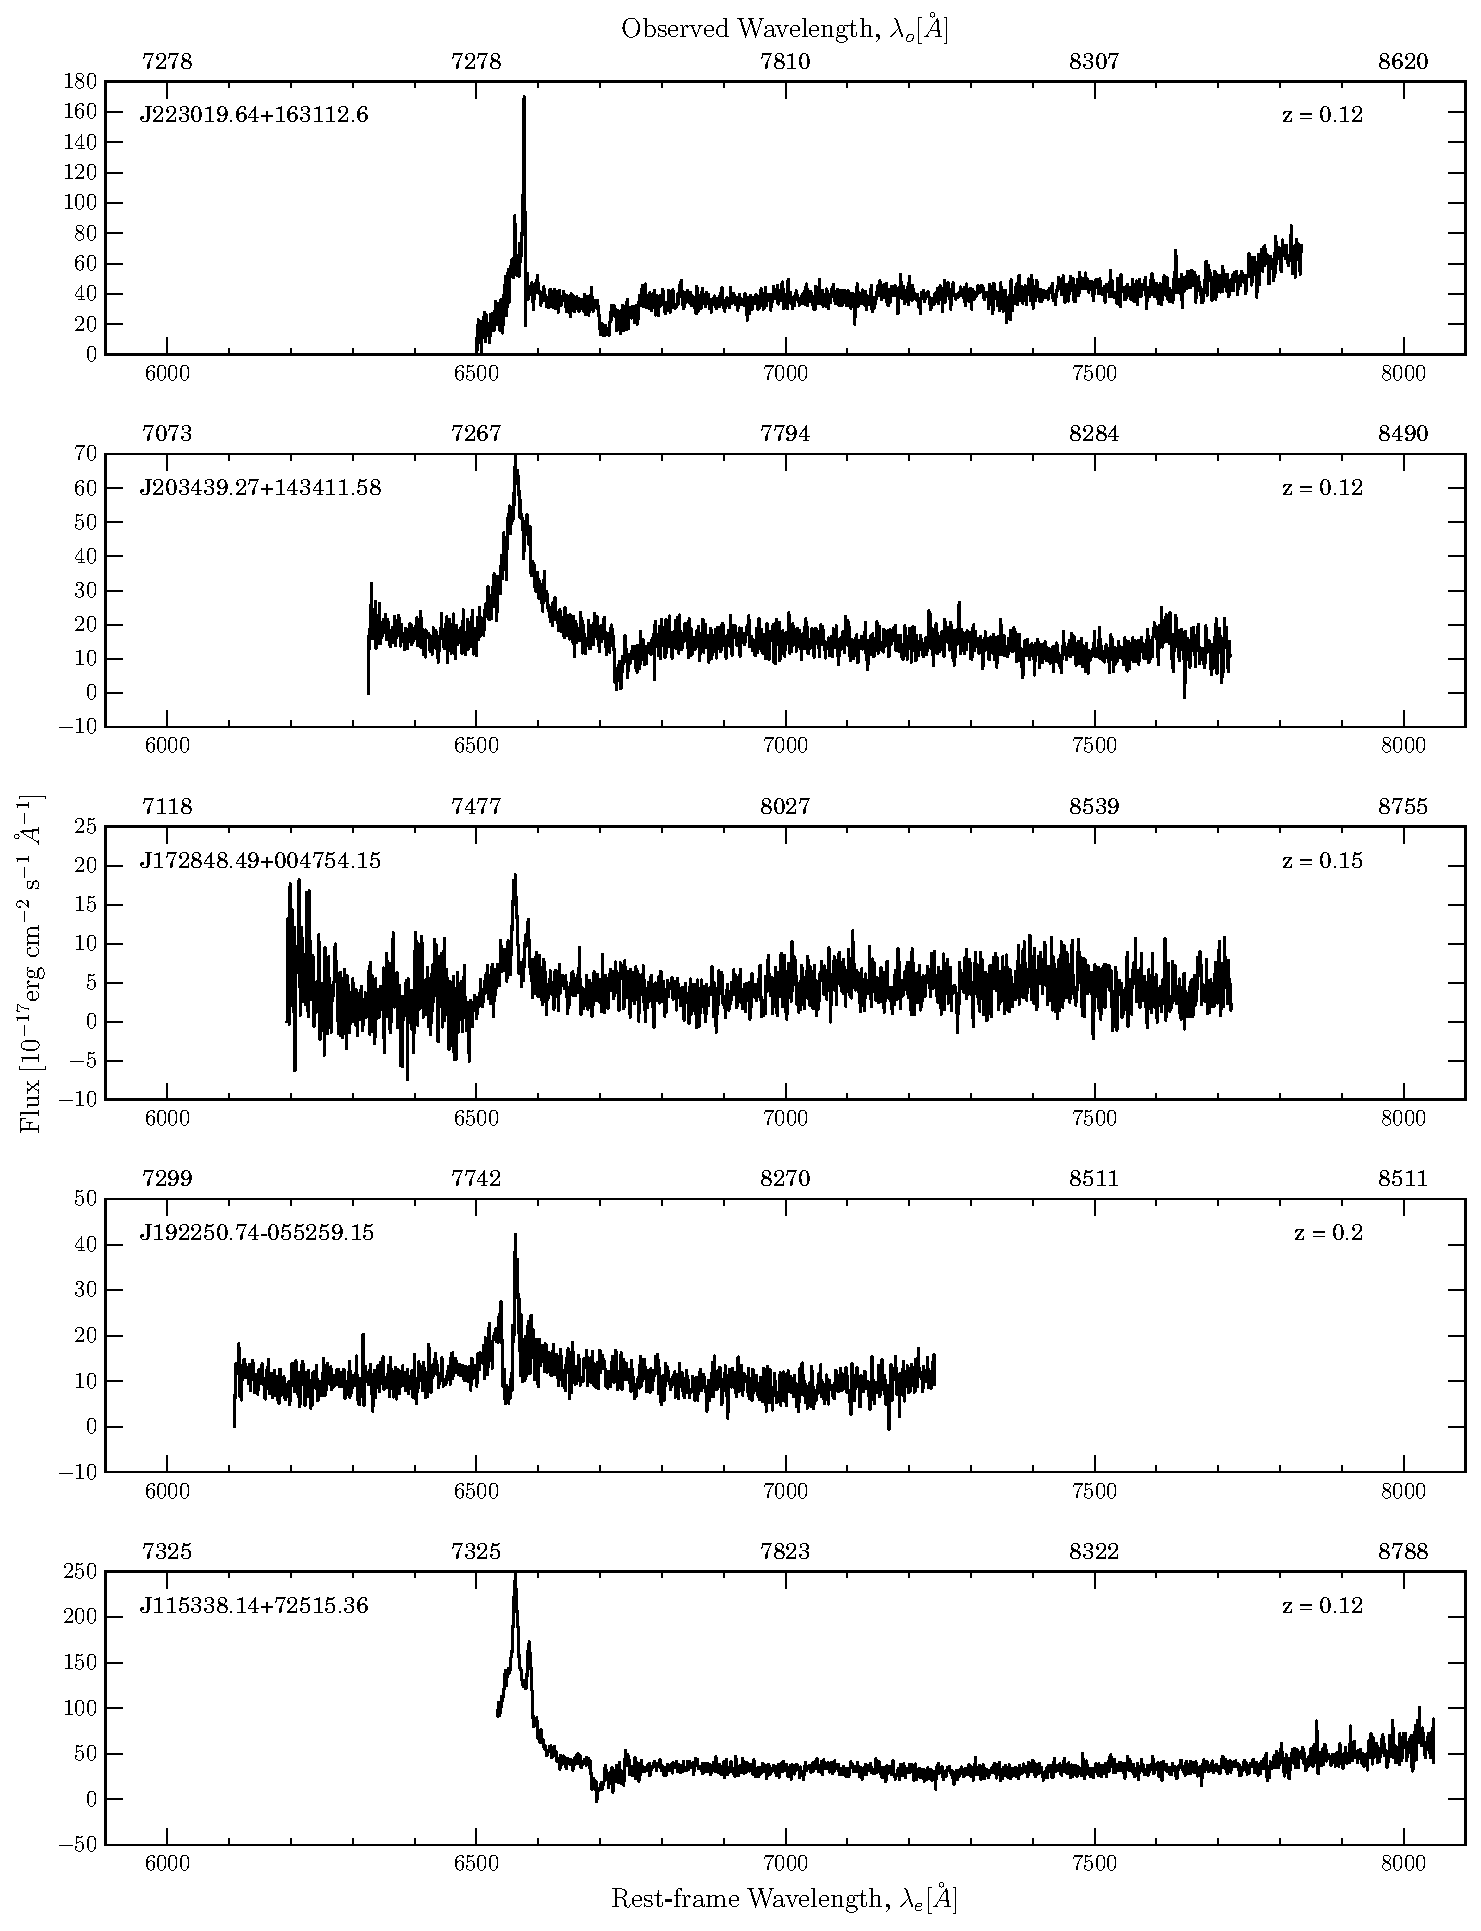
\includegraphics[width=\textwidth]{agn/int_spectra.pdf}
\caption[Optical spectra of 5 bulgeless galaxies observed on the INT with the IDS]{
Reduced spectra from the IDS on the INT for the 5 galaxies observed with the corresponding measured redshift values shown. Each panel shows the same rest-frame wavelength range (bottom axis of each panel); observed wavelengths are shown on the top axis of each panel, with redshifts in the top right of each panel. All spectra show broadened \ha\ emission, confirming that the multi-wavelength AGN selection employed here efficiently selects unobscured AGN.
}}
\label{fig:INTspectra}
\end{figure*}



% maybe some details about the spectral resolution?

Figure \ref{fig:redshifts} shows the redshift distribution of all 101 sources for which we have spectra; the mean redshift of the sample is $\left< z \right> = 0.129$, with the highest-redshift source having $z = 0.244$. 


\begin{figure}
\centering{
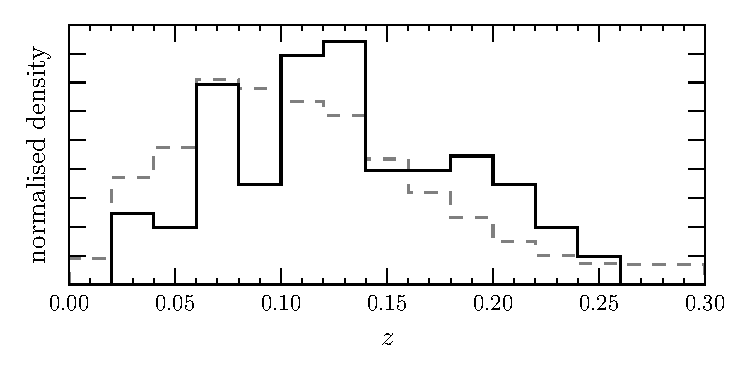
\includegraphics[width=0.9\textwidth]{agn/z_distribution_101_sdss.pdf}
\caption[Redshift distribution of bulgeless galaxies]{Normalised redshift distribution for all 101 sources (solid) for which we have spectra, either from SDSS or measurements with the IDS on the INT. Also shown is the overall redshift distribution of SDSS DR7 in the relevant redshift range of our sources (dashed).
}}
\label{fig:redshifts}
\end{figure}






%%%%%%%%%%%%%%%%%%%%%%%%%%%%%%%%%%%%%%%%%%%%%%
%
%
\subsection{Stellar and Black Hole Masses}\label{sec:masses}
%
%
%%%%%%%%%%%%%%%%%%%%%%%%%%%%%%%%%%%%%%%%%%%%%%

{\notebsm Probably want a short intro paragraph here. We compute masses because we want to explore co-evolution, below we describe how we do that. etc. Just something to keep the narrative going and prevent the section and subsection headings from colliding.}

%%%%%%%%%%%%%%%%%%%%%%%%%%%%%%%%%%%%%%%%%%%%%%
\subsubsection{Galaxy and bulge stellar masses}\label{sec:galmass}
%%%%%%%%%%%%%%%%%%%%%%%%%%%%%%%%%%%%%%%%%%%%%%

We calculate stellar masses using the well-studied relation between stellar mass, absolute galaxy $r$-band magnitude, and $u-r$ galaxy colour {\notebsm \citep[corrected for galactic extinction;][]{schlegelmapsorwhatever}}, following the method of \citet{baldry06}. We remove the AGN contribution to the luminosity and colour of each galaxy by subtracting the flux in the SDSS {\tt psfMag} from the flux in {\notebsm {\tt modelMag}}. {\tt psfMag} is the best estimate of unresolved emission, while {\tt modelMag} is the optimal quantity for computing aperture-matched source colours\footnote{https://www.sdss3.org/dr10/algorithms/magnitudes.php}. 
% not sure if this modelMag vs petroMag vs cModelMag will also be in e.g. Strauss et al. (2002)... must find someone to ask

The full sample of total stellar masses spans the range from {\notebsm $7 \times 10^9 \mmsun < M_* < 2 \times 10^{11} \mmsun $}, with a mean galaxy stellar mass of {\notebsm $12345 \mmsun $}. Each individual mass has an uncertainty of {\notebsm $0.3$ dex} from the scatter in the colour-luminosity relation, with typically an additional {\notebsm ????} uncertainty due to the AGN subtraction \citep[dependent on the nuclear luminosity, e.g.][]{simmons08}. The typical combined uncertainty in the stellar mass is {\notebsm ????} dex.

The nuclear emission, as estimated via comparison of {\tt psfMag} to {\tt modelMag}, is generally between {\notebsm 20 to 200 per cent} of the galaxy-only emission. The presence of the luminous AGN severely compromises the estimates of the bulge-to-total ratio in the host galaxy provided by, e.g., the {\tt fracDeV} parameter reported in the SDSS catalogs. That parameter estimates that 80 per cent of the galaxies in this sample are pure \citet{devaucouleurs} bulges in the $r$-band, despite the fact that the sample was selected on the basis of clear visual signatures of dominant disks (Figure \ref{fig:exampleimages}). None of the photometric parameters measured by the SDSS pipeline allow for the dual presence of an AGN and a host galaxy; without such considerations the unresolved AGN light is likely to be attributed to the compact bulge component in a bulge-disk model fit \citep{simmons08,thatothersimspaper,koss11}.

% wherever the first mention of a pseudo-bulge is, need to \citep{kormendy04}.
AGN-host decomposition based on 2-dimensional image fitting \citep[e.g.,][]{peng02,peng10,gim2d} is more reliable \citep[e.g.][]{mclure99,urry00,mclure01,sanchez04,pierce07,gabor09,simmons11,simmons12b,simmons13,koss11,schawinski12}, although even in high-resolution \emph{Hubble Space Telescope (HST)} images \citep{simmons08,thatothersimspaper} or SDSS imaging at $z \gtrsim 0.06$ \citep{koss11,simmons13} the recovered bulge-to-total ratio can be highly uncertain, particularly for disk-dominated galaxies with a small bulge or pseudo-bulge component. While the AGN-host decompositions of the sample of \citet{simmons13} recovered reliable parameters to compact pseudo-bulge components for 11 of 13 galaxies, those sources are at substantially lower redshift than this sample, and their AGN are significantly less luminous {\notebsm (quantify this more)}. 

We undertook a similar procedure as in that study to attempt bulge-to-total fits to 5 exemplar galaxies in this sample (Figure \ref{fig:exampleimages}), with a median redshift of {\notebsm $z = 0.13$} and typical $r$-band nuclear fluxes {\notebsm approximately equal to the total galaxy $r$-band flux}. We recovered stable, but highly uncertain, bulge-to-total ratios for only {\notebsm 2} of the 5 galaxies; in the remaining cases the nuclear emission is too bright and the resolution too low for a reliable bulge-to-disk decomposition. Detailed AGN-host fits to the SDSS images in the entire sample are not likely to produce useful measurements of bulge masses; \emph{HST} imaging, which would enable this, is currently not available for the galaxies in this sample.

Nevertheless, it is possible to constrain the bulge contribution to the host galaxies using existing structural parameters from large-scale studies performing bulge-disk decompositions of SDSS galaxies. While such studies do not account for the presence of an AGN, their tendency to overestimate the bulge-to-total ratio as a result means that bulge masses derived from these quantities may be taken to be conservative upper limits.

We use the bulge-disk decompositions of \citet{simard11}, who fit multiple models to 1.12 million galaxies in the SDSS catalog and determined best-fit models and structural parameters for each. We take the $r$-band bulge-to-total ratio {\notebsm of the best-fit model} as an upper limit to the true bulge-to-total ratio of these AGN host galaxies. To convert limits on bulge luminosities to limits on bulge masses, we assume the mass-to-light ratio of the bulge is equal to the mass-to-light ratio of the disk. In disk-dominated galaxies, where many of the ``bulge'' components are likely to be rotationally-supported pseudo-bulges \citep{kormendy04} whose stellar populations are similar to that of the disk {\notebsm \citep[e.g.,][]{graham01a,atheorypaperonthis}}, this is a reasonable assumption.

The upper bulge-to-total limits of the 89 galaxies in this sample which were included in the \citeauthor{simard11} study range from {\notebsm $0.13 \leq \left({\rm B/Tot}\right)_{\rm max} \leq 1.0$, with a mean value of 0.5}. Applying these bulge-to-total limits to the stellar masses computed using the colour-luminosity relation \citep{bell01,baldry06} results in bulge mass upper limits of {\notebsm $3 \times 10^9 \mmsun < {\rm M_{bulge}} < 7 \times 10^{10} \mmsun $}. These mass limits will be compared with black hole masses for the sample in Section \ref{sec:bhmassrelations}.


%%%%%%%%%%%%%%%%%%%%%%%%%%%%%%%%%%%%%%%%%%%%%%
\subsubsection{Black hole mass estimates}\label{sec:bhmass}
%%%%%%%%%%%%%%%%%%%%%%%%%%%%%%%%%%%%%%%%%%%%%%

The selection of unobscured AGN facilitates accurate estimates of black hole masses. Unobscured AGN have broad emission lines originating from within the black hole sphere of influence, which can be used to estimate the velocity of the orbiting broad-line clouds and the radius of the emitting region \citep{somecanonicalpapers,areviewpaper}. Each AGN in the sample has 1 spectrum, meaning the broad-line-derived black hole masses are ``single-epoch'', relying on simplifying geometric assumptions and empirically established relationships between observed and physical quantities to compute masses using the virial theorem \citep{greene,others}. Single-epoch black hole mass estimates are more uncertain than those derived from reverberation mapping and other more precise methods \citep{Barthetal_maybe,also_we_should_totally_cite_LIGO_lolz}, but they are considerably more accurate than many other methods (e.g., Eddington-based estimates). We use the established relation between black hole mass and the FWHM and luminosity in the broad \ha\ line \citep{gh07a}.

We perform spectral fitting on each of the SDSS and INT spectra described in Section \ref{sec:spectra} to recover narrow-line strengths and broad-line strengths and widths to the $\mha\ 6563$ \AA\ line, using \gandalf\ \citep{sarzi06} {\notebsm to fit multiple simultaneous lines as well as the continuum}. \gandalf\ is optimised for use with SDSS spectra; using the program with the INT spectra required minimal data re-formatting: we binned logarithmically and de-redshifted the spectra. {\notebsm From the continuum-subtracted best fit}, we determine the FWHM and line flux of the broad \ha\ line simultaneously with the narrow \ha\ component via \emcee\footnote{\url{dan.iel.fm/emcee/}}, a Python implementation of a Markov Chain Monte Carlo \citep[MCMC;][]{mackay03, gw10} affine invariant ensemble sampler by \cite{emcee13}. 

The uncertainties reported by \emcee\ are limited to those from the separation of narrow and broad line components in measurement of the FWHM. {\notebsm We also determine uncertainties from the \gandalf\ fits using a bootstrap method sampling within the spectral noise and re-fitting with $N=1000$ iterations for each spectrum.} The reported uncertainties on black hole masses include both these sources of uncertainty as well as the reported uncertainties in the black hole-broad line relation \citep{gh07a}. There are other sources of uncertainties, such as those involved in implicitly assuming a fixed geometric correction factor $f$ for each SMBH, and the error introduced by assuming a Gaussian line profile for all measured broad lines. Determining uncertainties for the former is outside the scope of this study; based on visual inspection of the line fits the latter is very small {\notebsm (not sure how to estimate how small? Could try it out on the fits with the worst non-artifact residuals?)} compared to the other uncertainties. The fits to the INT spectra are shown in Figure \ref{fig:zoomspectra}.

The black hole masses for the sample of ??? galaxies range from {\notebsm $10^6 \mmsun \leq \mmbh \leq 2 \times 10^9 \mmsun$. The median mass is $3 \times 10^7 \mmsun$}. We compare these to galaxy stellar masses and bulge mass upper limits in Section \ref{sec:bhmassrelations}.






\begin{figure}
\centering{
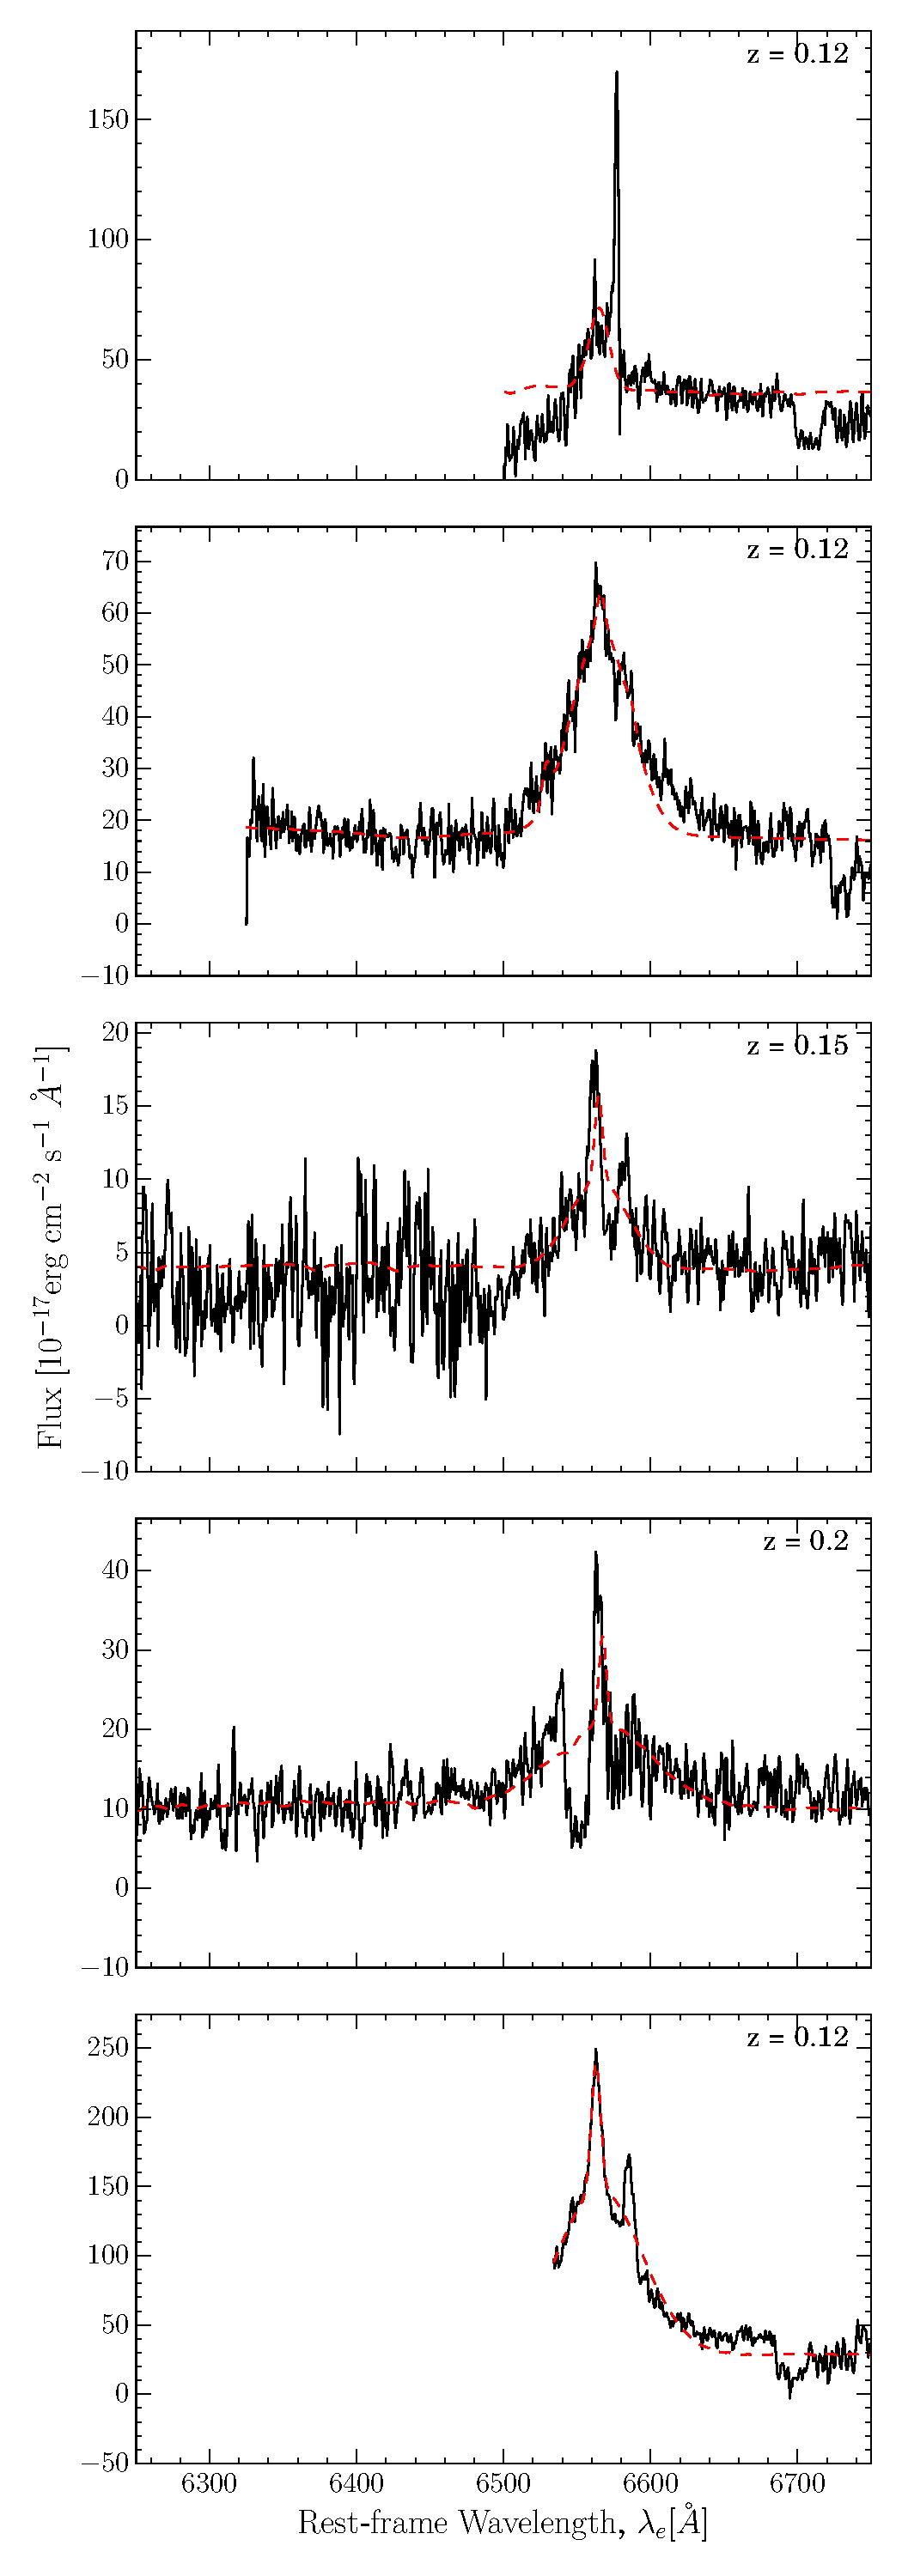
\includegraphics[height=0.9 \textheight]{agn/int_zoom_spectra.pdf}}
\caption[Zoom in on $H\alpha$ region of the spectra of 5 galaxies observed with the IDS on the INT]{
Reduced spectra from the IDS on the INT for the 5 galaxies observed with the corresponding measured redshift values shown. Spectra are aligned with the broad $H\alpha$ emission line, the gaussian fits to which are shown by the dashed red line.  
}
\label{fig:zoomspectra}
\end{figure}



%%%%%%%%%%%%%%%%%%%%%%%%%%%%%%%%%%%%%%%%%%%%%%
%
%  
\subsection{Galaxy-Black Hole Mass Relations}\label{sec:bhmassrelations}
%
% 
%%%%%%%%%%%%%%%%%%%%%%%%%%%%%%%%%%%%%%%%%%%%%%

\begin{figure*}
\centering{
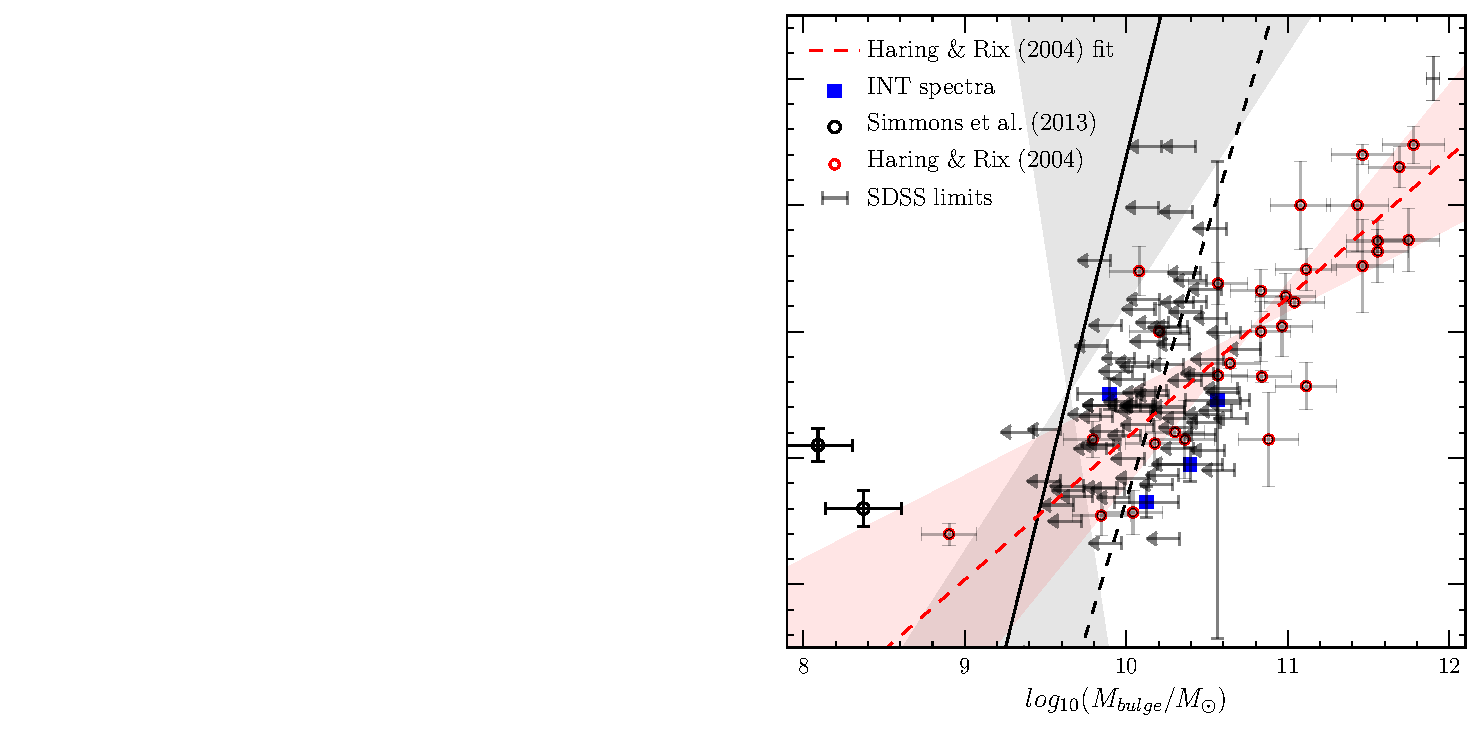
\includegraphics[width=\textwidth]{agn/mass_bh_total_mass_fit_with_bulge_limits_INT_simmons13_measurements_linmix_fit.pdf}
\caption[Black hole bulge mass and stellar mass relations for the bulgeless AGN sample]{Total stellar mass against the black hole mass (left) of the 101 galaxies, including those observed by SDSS (crosses), with the IDS on INT (blue squares) and detections from \citet[open cirlces]{simmons13}. The best fit line to the data points and two-dimensional errors from linear regression is shown (solid line) with $\pm3\sigma$ (grey shaded). For 89 of the galaxies we have upper limits (black arrows) on the $(\rm{B/T})_g$ ratio from which we can determine an upper limit on the stellar bulge mass. We plot this value against the black hole mass (right) and show the best fit to these upper limits and two-dimensional errors using linear regression methods (solid line) with $\pm3\sigma$ (grey shaded). The dashed line shows the fit if the upper limits are not treated as such. In both panels we also show the best fit found using this same method to the early-type galaxies of \citet{haringrix04} (dashed line) with $\pm3\sigma$ (red shaded) and the measured values shown by the red circles. Despite the fact that these galaxies are predominantly disk dominated they will are most likely to lie above the \citet{haringrix04} relationship found for bulge dominated systems (see discussion in Section \ref{sec:bhmassrelations}).
}}
\label{fig:totvsbh}
\end{figure*}


 
The total stellar mass (estimated bulge masses - see Section \ref{sec:galmass}) and black hole masses of the 101 galaxies in our sample are shown in the left (right) panel of Figure \ref{fig:totvsbh}. We fit a linear regression model to both of these relations using a Bayesian method which encompasses both the two-dimensional uncertainties on each measurement and the intrinsic scatter in the data. This method is outlined in \citet{kelly07} and is publicly available as a \emph{Python} module \textsc{linmix}\footnote{\url{http://linmix.readthedocs.org/}}. For the bulge mass in the right panel of Figure \ref{fig:totvsbh} this method can also incorporate the upper limits on the measurements for the 89 SDSS galaxies (see Section \ref{sec:galmass}. 

Using this same method, we fit to the observations of 30 early-type galaxies from \citet{haringrix04}. Despite the fact that our sample of galaxies is disk dominated and contain either a pseudo-bulge or no bulge, they most likely lie above the relationship derived using the bulge dominated galaxies of \citet{haringrix04}. 

We consider how the black hole mass compares to the Eddington ratio, or accretion rate of these disk dominated galaxies and compare with a redshift matched subsample of 198 galaxies in the DR7 quasar sample from \citet{shen11}. This is shown in Figure \ref{fig:mbhvsbol}. The 101 galaxies in our disk dominated sample have both lower black hole masses and lower bolometric luminosities in comparison to the \citet{shen11} sample, however the Eddington ratio's are very similar, see Figure \ref{fig:eddratioshen}. In fact, the Eddington ratio's of the redshift matched sample are on average, lower than that for the disk dominated sample. We can reject the null hypothesis that the disk dominated galaxies are drawn from the same distribution as the redshift matched quasar sample from \citet{shen11} but not for the entire quasar sample of \citet{shen11}. {\notebsm 'ERE BE SCIENCE!}

Within this redshift matched sample, 108 galaxies were morphologically classified by the Galaxy Zoo 1 project \cite{lintott08, lintott11}, all of which have a debiased combined spiral vote fraction (Galaxy Zoo 1 did not ask whether a galaxy was a disk, therefore we can approximate the combined spiral vote fraction as a disk vote fraction) of $p_{CS} < 0.5$ and mean value of $\left<p_{CS} \right> = 0.17$. 

Slightly higher accretion rates are therefore occurring in the AGN of these disk dominated galaxies than in a bulge dominated quasar sample from SDSS. {\notebsm 'ERE BE SCIENCE!}. 

\begin{figure}
\centering{
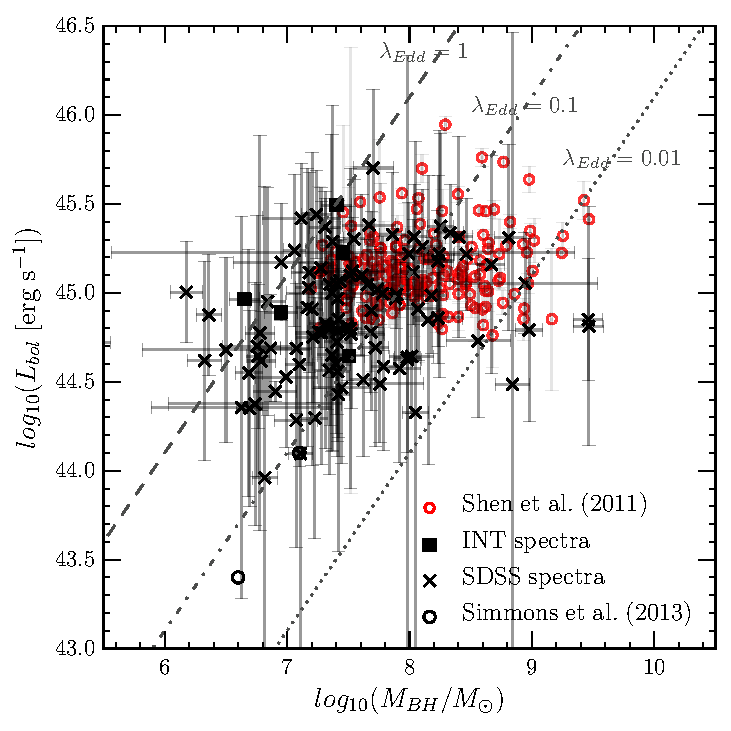
\includegraphics[width=\textwidth]{agn/mass_bh_bol_luminosity_with_all_errors_shen_11.pdf}}
\caption[Black hole mass against luminosity for the bulgeless AGN sample]{Black hole mass against bolometric luminosity for the 101 galaxies, including those observed by SDSS (crosses) and with the IDS on INT (squares). We also show detections from {\notebsm Simmons et al. (2013)} (open circles) and those from the redshift matched sample of {\notebsm Shen et al. (2011)}. For reference we show lines of example Eddington ratios of $\Lambda_{Edd}$ = 1 (dashed),  $\Lambda_{Edd}$ = 0.1 (dot-dashed) and $\Lambda_{Edd}$ = 0.01 (dotted).
}
\label{fig:mbhvsbol}
\end{figure}

\begin{figure}
\centering{
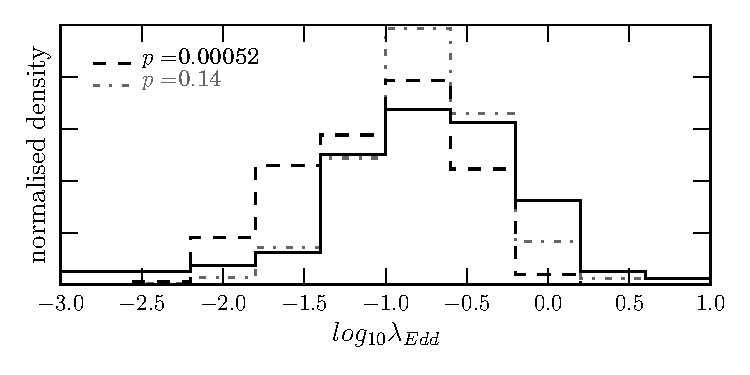
\includegraphics[width=0.8\textwidth]{agn/edd_ratio_z_matched_shen_2011_compare.pdf}}
\caption[Eddington ratio distribution of the bulgeless AGN sample]{Normalised distributions of logarithmic Eddington ratio for the sample of 101 disk dominated galaxies (solid line), compared with that for the redshift matched sample from Shen et al. (2011; dashed line) and the entire sample (dot-dashed line) We also provide the p-values of a 2 sample KS test between the disk dominated sample and each of the quasar samples. We reject the null hypothesis that the two samples are drawn from the same population for the redshift matched quasar sample but accept the null hypothesis for the entire quasar sample of \citet{shen11}.  
}
\label{fig:eddratioshen}
\end{figure}


%%%%%%%%%%%%%%%%%%%%%%%%%%%%%%%%%%%%%%%%%%%%%%
%
%  
\subsection{Discussion}\label{sec:discussion}
%
%
%%%%%%%%%%%%%%%%%%%%%%%%%%%%%%%%%%%%%%%%%%%%%%

\begin{itemize}
\item Eddington ratios - use WISE W3 for Lbol and compare with BH masses to talk about Eddington ratios of the sample in Figure \ref{fig:mbhvsbol}.


\item Do the Lbol or Eddington ratios or masses look different for disk-dominated hosts in clear interactions?

\end{itemize}


